\documentclass[12pt]{report}
\title{\textbf{\Huge View Maintenance \\ in Data Warehousing } }
\author{CV Hariharan \bullet 1610110147 \\ Divya Raj \bullet 1610110123 \\ Devansh Purohit \bullet 1610110116}
\date{}

\usepackage[margin=1.4in]{geometry}
\usepackage{graphicx}
\usepackage{enumitem}
\usepackage{xcolor}
\usepackage{float}
\usepackage{amsmath}

\begin{document}
\maketitle
\section*{Acknowledgment}
We would like to thank Dr. Sonia Khetarpaul, our instructor for the Advance Database Management course this semester, for helping us with this project and the report. She taught us the concepts needed for this project and was available to us for help, whenever we needed it. Thank you.\\
\\We would also like to thank Hemant Jain and Anjana Gosain for their amazing paper titled "A Comprehensive Study of View Maintenance Approaches in 
Data Warehousing Evolution". It was a source of great help throughout this project. \\
\\Also, huge gratitude towards Abdulaziz S. Almazyad and Mohammad Khubeb Siddiqui for their paper titled "Incremental View Maintenance: An Algorithmic 
Approach". It gave us great insight into the incremental approach to view maintenance and inspired the final solution that we implemented.
\\\\Finally, we would like to thank Github user AntonioL for his repository -  "factorized-incremental-maintenance". It provided us a code wise basis for the project and helped us get started.
\\\\All the relevant links can be found at the end of this report in the Bibliography section.
\tableofcontents
\newpage
\renewcommand{\thesection}{\arabic{section}}
\section{Introduction}
A data warehouse mainly stores integrated information over data from 
many different remote data sources for query and analysis. The 
integrated information at the data warehouse is stored in the form of 
materialized views. Using these materialized views, user queries may be 
answered quickly and efficiently as the information may be directly 
available. These materialized views must be maintained in answer to 
actual relation updates in the different remote sources. \\
One of the issues 
related to materialized views is that whether they should be recomputed 
or they should be adapted incrementally after every change in the base 
relations. \\
View maintenance is the process of updating a materialized 
view in response to changes to the underlying data is called view 
maintenance. There are several algorithms developed by different 
authors to ease the problem of view maintenance for data warehouse 
systems. \cite{basic} \\
In this report, we document the already existing approaches in the field, describe the approach that we took and also show our findings and conclusions. 
\\\\First, some definitions-

\begin{description}[font=$\bullet$~\normalfont\scshape\color{orange!50!black}]
\item [Source] - A  database,  application,  file,  or  other  storage  facility  from which  the  data  in  a  data  warehouse  is  derived.  The  source contains  the  operating  data,  flat  files  and  stage  files.  The  
stage  file  receives  the  data  from  source  process  and  it  
verifies  its  credit-ability  and  the  required  data  files  will  be  
passed   to   warehouse   through   view   manager.   Source   
division also termed as top tier of architecture. \cite{saudi}
\item[Warehouse] - A relational database that is designed for query and analysis rather   than   transaction   processing.   A   data   warehouse
usually   contains   historical   data   that   is   derived   from transaction data, but it can include data from other sources. It  separates  analysis  workload  from  transaction  workload  and  enables  a  business  to  consolidate  data  from  several
sources.  It  contains  the  Summary  data,  raw  data,  metadata,
mined  data  etc.  Warehouse  division  also  termed  as  middle
tier of architecture. \cite{saudi}
\item[User] - Users   may   be   end   users   and   make   use   of   the   data warehouse   view   maintenance   in   the   Analysis   of   Data   
mining, Data reporting etc, and User division also termed as 
top tier of the architecture. \cite{saudi}
\end{description}

\section{Existing and Related Work}
Various  approaches  have  been  introduced  for  maintaining  
the view in a warehouse environment. 
\begin{figure}[H]
\centering 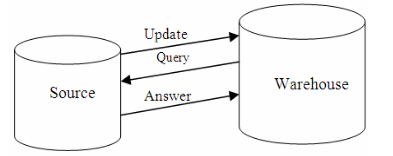
\includegraphics[width=0.7\textwidth]{images/pic1.png}
\caption{Basic Approach}
\end{figure}
\begin{description}[font=$\bullet$~\normalfont\scshape\color{blue!50!black}]
\item[Basic Algorithm] In Fig 1, it is shown that there 
is communication between Source and  the  warehouse,  when  update  occurs  at  source,  it  sends the  notification  to  warehouse  later  on  warehouse  sends  the query  to  source  for  the  corresponding  update  as  source  
receives the query it sends the answer to warehouse to that corresponding query.\\
\\1. When  an  update  occurs at  the  source,  it  sends  the update notification to the warehouse. 
\\2. Warehouse  receives  the  notification  and  sends  
back the query to the source about the update. 
\\3. Source receives the query    sent    by    the    
warehouse and returns the answer to that query.  
\\\\The   basic   algorithm   is   neither   convergent   nor   weakly   
consistent in warehouse environment. \cite{saudi}
\item[Recompute View] RV does not rely on incremental view maintenance 
approach. It is based on recomputation of materialized view 
from the scratch. When ever the update occurs at the source 
it recomputes the view from the scratch. In RV approach 
warehouse sends the Query to the source asking it to 
recompute the view from the scratch after certain number of 
updates. RV sends 2 messages for each update. The bytes 
transferred are much higher
 in RV than the relative 
algorithms. \\This degrades the performance of RV \cite{saudi}
\\\item[Eager Compensating Algorithm]
COLLECT =  
\\W $up_i$
: receive $U_i$; 
\begin{center}
Let $Q_i$
= v($U_i$) – 
$_{Q}\in_{UQS}Q_j(U_i) $
\\send $Q_i$ to the source; 
\\trigger event S $qu_i$ at the source 
\end{center}
W $ans_i$: receive $A_i$; 
\begin{center}
        let COLLECT = COLLECT + $A_i$; 
\\        if UQS =
           \\then { MV ←MV + COLLECT; COLLECT ←} 
\\        else do nothing. 
\end{center}
ECA is an incremental view maintenance algorithm. It is a 
method   for   fixing   the   view   maintenance   problem   that   
occurs  due  to  the  decoupling  between  base  data  and  the  
view maintenance manager at the warehouse. The key idea 
of  the  ECA  algorithm  is  that  it  cannot  rely  on  the  state  of  
the     base     information     that     is     continuously     being     
updated/modified  by  the  sources.  It  must  keep  track  of  the  
updates  received  from  the  source  and  then  filter  out  i.e.,  
compensate any information that will duplicate the resulting 
queries. By subtracting (or adding) the results it knows that 
will (not) get in future queries, it will create an accurate end 
result for the view.
\\The above algorithm states that: 
Initially  the  COLLECT  will  be  empty,  source  executes  an  
update  ($U_i$)  and  the  notification  sent  to  the  warehouse.  
Warehouse  receives  the  source  update ($U_i$)  and  sends  the  
query ($Q_i$)     based on  ($U_i$), for each query in     
UQS(Unanswered Query Set: the set of query set that were 
sent by the warehouse, but answers have not been received)
formulates  a  compensating  Query $Q_j$ based on $U_i$ and $Q_i$ with $Q_j$. Warehouse receive the query result and update the 
Materialized  View(MV),  the  result  of  the  query  should  be  
applied to the Materialized Vi
ew(MV) only after the answer 
to this query and all related compensating query have been 
received. 
To   avoid   invalid   state   ECA   collects   the   intermediate   
answers  in  relation  denote
d  as  COLLECT  (initially  its  
empty).\cite{saudi}
\item[Lazy Approach] Lazy approach maintains the view in a lazy manner that 
relieves the updates of the maintenance overhead as in the 
incremental view maintenance approaches. View 
maintenance is postponed unt
il the system has free cycles 
or it is referenced by any query. These free cycles are utilized for the view maintenance that relieves the updates 
and queries from the overhead
. The updates are combined 
from different transactions into a single maintenance task. It 
also exploits row versioning. In lazy maintenance the 
updates do not maintain the view it just stores the required 
information so that the affect
ed views can be maintained 
later. It actually uses system free cycles to maintain the 
views, in this no updates or queries pay for the maintenance 
task. But, in case the view is not
 up to date and query is sent 
over it, then the particular query has to pay for all part of 
the view maintenance and some
delay also. However, it 
pays only the view maintenance that it uses and not for 
other views \cite{basic}
\end{description}
\section{Proposed Approach}
Fuel is an important resource. Any plant which depends extensively on fuel needs to store it somewhere from where it could be used later on when the supply of fuel from the mine is improper. This is where a fuel storage facility comes into picture. \par In a thermal power plant, the first step in process of power generation is that the fuel is brought to breaker house with the help of belt conveyor, here light dust is separated with the help of rotary machine through the action of gravity. It further goes to the crusher where it is crushed to a size of about 50mm.
\section{Implementation and Results}
The water that has been converted to steam, is brought to the turbines under high pressure. This steam is used to rotate them. Normal water is taken from the river, and it contains a lot of dirt, suspended particulate matter (SPM), dissolved minerals and dissolved gases such as air etc. If the water fed to the boiler is not treated, it will reduce the life and efficiency of equipment by corroding the surfaces which may lead to overheating of pressure parts and explosions. \par This particulate matter is separated out by adding {\it alum} into the water. Alum coagulates the dirt and increases its density. Then, due to gravity, this coagulated matter settles down in the water which is then removed from it. 


\par After gravity separation, water softening is done by ion exchange process. As the hardness comes through the carbonates and bicarbonates of sodium and magnesium, these salts are removed from water anion exchange and cation exchange process. \par Water also contains dissolved oxygen and this leads to corrosion and fouling of boiler tubes and surfaces when it comes in their contact. So removing dissolved oxygen from water is done by adding oxygen scavengers and by using a Deaerator tank. Deaerator tank also acts as a feed water tank to store the feed water. On heating feed water in a deaerator tank decreases the solubility of air in water, thereby removing the dissolved air from the water.
\section{Conclusions and Limitations}
A boiler is a high pressure vessel used to generate high pressure steam at saturated temperatures. Water tube boiler consists of a furnace enclosed by the water tubes membrane. The crushed fuel from the crushers is fed into the boiler furnace over the grate. The hot air from the Forced Draft (FD) fan is mixed with the crushed fuel causing combustion of fuel.
Combustion of fuel generates a lot of radiation heat which is transferred to water in the membrane tubes. Flue gases generated during combustion travel at high velocity across the convection bank of tubes thereby heating water through convection heat transfer. Hot water is sent to a boiler drum at high pressure through the feed water pump. The boiler tubes which are in contact with low temperature acts as downcomers to circulate the water while the tubes which are in contact with high temperature acts as risers to carry steam. This leads to an effective circulation of water thereby preventing the tubes from getting overheated.

Steam leaving the boiler is at a saturated temperature and pressure but there are a lot of heat losses during its transportation to the turbines. So to increase the quality of steam, steam Superheater is installed in a radiative section of a boiler to increase its temperature and dryness fraction without increasing its pressure as well as to accommodate for the transportation temperature losses.

The exhaust gases leaving the boiler are generally at high temperature and this waste heat is extracted by installing an Economiser or Water Pre heaters to preheat the feed water to the boiler and Air Preheaters to pre-heat the air coming from the Forced Draft Fan required for the combustion of fuel. Installing this equipment help to decrease the flue gas temperature thereby increasing the efficiency.

The flue gases leaving the boiler also contain some ash particles, so to reduce the air pollution, flue gases are allowed to pass through the Dust Collectors and Bag Filters to remove the ash particulates from the flue gases and are sometimes passed through the Wet Scrubbers to decrease the sulfur content from the gases.

The flue gases are drawn through this equipment using an Induced Draft (ID) Fan which is designed for a fixed capacity and head to prevent any back pressure. After the ID fan, flue gases are exhausted off into the atmosphere using a chimney.
\\ 
\begin{thebibliography}{999}
\bibitem{saudi}
Abdulaziz S. Almazyad and Mohammad Khubeb Siddiqui\emph{ Incremental View Maintenance: An Algorithmic 
Approach}.
 	 Feb, 2016.
\bibitem{basic}
Hemant Jain Anjana Gosain \emph{A Comprehensive Study of View Maintenance Approaches in Data Warehousing Evolution }.
 	 Sept, 2012. 	 
\end{thebibliography}
\end{document}